We present a new logic: Temporal Stream Logic (\TSL), which is
especially designed for synthesis and allows for the manipulatation of infinite
streams of arbitrary (even non-enumerative, or higher order) type. It
provides a straightforward notation to specify how outputs are
computed from inputs, while using an intuitive interface to access
time. The main focus of \TSL is to describe temporal control
flow, while abstracting away concrete implementation details. This not
only keeps the logic intuitive and simple, but also allows a user to identify
problems in the control flow even without a concrete implementation at
hand. In this way, the use of \TSL scales up to any required abstraction, such as API
calls or complex algorithmic transformations.

\medskip

\noindent \textit{Architecture} A TSL formula~$ \varphi $ specifies a
reactive system that in every time step processes a finite number of inputs~$ \inames $
and produces a finite number of outputs~$ \onames $. Furthermore, it
uses cells~$ \cells $ to store a value computed at time~$ t $,
which can then be reused in the next time step~$ t + 1 $. An overview
of the architecture of such a system is given in \cref{fig:tslarchitecture}. In terms
of behavior, the environment produces infinite streams of input data,
while the system uses pure (side-effect free) functions to transform
the values of these input streams in every time step. After their
transformation, the data values are either passed to an output stream
or are passed to a cell, which pipes the output value from one time step back to the corresponding input value of the next.
The behaviour of the system is captured by its infinite execution over time.

\begin{figure}[t]
  \centering

  \begin{subfigure}[b]{0.58\textwidth}
  \begin{tikzpicture}[scale=0.8]

    \node[anchor=east,inner sep=0pt] at (-2.8,-1.5) {
      \small
      \begin{tabular}{c}
        inputs: \\[0.1em] $ \inames $
      \end{tabular}
    };

    \node at (0,1.38) {
      \small
      cells: $ \cells $
    };

    \node[anchor=west,inner sep=0pt] at (2.8,-1.5) {
      \small
      \begin{tabular}{c}
        outputs: \\[0.1em]
        $ \onames $
      \end{tabular}
    };

    \node at (0,0) {
      \begin{tikzpicture}[xscale=0.8,yscale=0.56]
        \node[fill, fill=blue!30,minimum height=5.5em, minimum width=10.5em] (C) {};

        \node at (C) {
          \small
          \begin{tabular}{c}
            \textit{reactive system} \\[0.4em]
            \textit{implementing a} \\[0.4em]
            \textit{TSL specification~$ \varphi $}
            \end{tabular}
        };

        \node[minimum size=0.9em] (H0) at (0,1.95) {};
        \node[minimum size=0.9em] (H1) at (0,2.6) {};
        \node[minimum size=0.9em] (H2) at (0,3.8) {};

        % signals
        \path[->,>=stealth,line width=0.7pt]
        ($ (C.west) + (-0.6,-1.3) $) edge ($ (C.west) + (0,-1.3) $)
        ($ (C.west) + (-0.6,-0.6) $) edge ($ (C.west) + (0,-0.6) $)
        ($ (C.west) + (-0.6,-0.3) $) edge ($ (C.west) + (0,-0.3) $)
        ($ (C.east) + (0,-1.3) $) edge ($ (C.east) + (0.6,-1.3) $)
        ($ (C.east) + (0,-0.6) $) edge ($ (C.east) + (0.6,-0.6) $)
        ($ (C.east) + (0,-0.3) $) edge ($ (C.east) + (0.6,-0.3) $)
        ;

        \node at ($ (C.west) + (-0.35,-0.85) $) {\scalebox{0.6}{$ \vdots $}};
        \node at ($ (C.east) + (0.25,-0.85) $) {\scalebox{0.6}{$ \vdots $}};

        % cells
        \draw[line width=0.7pt,-,>=stealth,gray]
        ($ (C.east) + (0,1.3) $) -- (2.7,1.3) |- (H0);
        \draw[line width=0.7pt,->,>=stealth,gray]
        (H0) -| (-2.7,1.3) -- ($ (C.west) + (0,1.3) $);

        \draw[line width=0.7pt,-,>=stealth,gray]
        ($ (C.east) + (0,1) $) -- (3,1) |- (H1);
        \draw[line width=0.7pt,->,>=stealth,gray]
        (H1) -| (-3,1) |- ($ (C.west) + (0,1) $);

        \draw[line width=0.7pt,-,>=stealth,gray]
        ($ (C.east) + (0,0.3) $) -- (3.6,0.3) |- (H2);
        \draw[line width=0.7pt,->,>=stealth,gray]
        (H2) -| (-3.6,0.3) |- ($ (C.west) + (0,0.3) $);

        \node at ($ (C.west) + (-0.35,0.75) $) {\scalebox{0.6}{$ \vdots $}};
        \node at ($ (C.east) + (0.25,0.75) $) {\scalebox{0.6}{$ \vdots $}};

        \fill[fill=orange!60]
        ($ (H0.north west) + (0,-0.1) $) --
        ($ (H0.south west) + (0,0.1) $) --
        ($ (H0.south west) + (0.1,0) $) --
        ($ (H0.south east) + (-0.1,0) $) --
        ($ (H0.south east) + (0,0.1) $) --
        ($ (H0.north east) + (0,-0.1) $) --
        ($ (H0.north east) + (-0.1,0) $) --
        ($ (H0.north west) + (0.1,0) $) --
        cycle;

        \fill[fill=orange!60]
        ($ (H1.north west) + (0,-0.1) $) --
        ($ (H1.south west) + (0,0.1) $) --
        ($ (H1.south west) + (0.1,0) $) --
        ($ (H1.south east) + (-0.1,0) $) --
        ($ (H1.south east) + (0,0.1) $) --
        ($ (H1.north east) + (0,-0.1) $) --
        ($ (H1.north east) + (-0.1,0) $) --
        ($ (H1.north west) + (0.1,0) $) --
        cycle;

        \fill[fill=orange!60]
        ($ (H2.north west) + (0,-0.1) $) --
        ($ (H2.south west) + (0,0.1) $) --
        ($ (H2.south west) + (0.1,0) $) --
        ($ (H2.south east) + (-0.1,0) $) --
        ($ (H2.south east) + (0,0.1) $) --
        ($ (H2.north east) + (0,-0.1) $) --
        ($ (H2.north east) + (-0.1,0) $) --
        ($ (H2.north west) + (0.1,0) $) --
        cycle;

      \end{tikzpicture}
    };
  \end{tikzpicture}
\caption{Architecture \mbox{\ }}
\label{fig:tslarchitecture}
\end{subfigure}
\begin{subfigure}[b]{0.41\textwidth}
  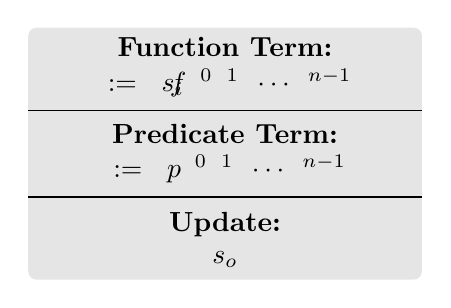
\begin{tikzpicture}

    \fill[gray!20,rounded corners=3] (-2.5,-2.5) rectangle (2.5,0.7);

    \node[anchor=center] at (0,0.45) {
      \textbf{Function Term:}
    };

    \node[anchor=center] at (0,0) {
      $ \fterm \ := \ \; \name{s}_{\name{i}} \! \! \sep \! \name{f} \ \, \fterm^{0} \
      \, \fterm^{1} \ \, \cdots \ \, \fterm^{n-1} $
    };

    \draw (-2.5,-0.35) -- (2.5,-0.35);

    \node[anchor=center] at (0,-0.65) {
      \textbf{Predicate Term:}
    };

    \node[anchor=center] at (0,-1.1) {
      $ \pterm \ := \ \;
      \name{p} \ \, \fterm^{0} \ \, \fterm^{1} \ \, \cdots \ \, \fterm^{n-1}  $
    };

    \draw (-2.5,-1.45) -- (2.5,-1.45);

    \node[anchor=center] at (0,-1.8) {
      \textbf{Update:}
    };

    \node[anchor=center] at (0,-2.25) {
      $ \upd{\name{s}_{\name{o}}}{\fterm} $
    };
  \end{tikzpicture}
  \caption{Term Definitions \mbox{\ }}
  \label{fig:termdefinitions}
\end{subfigure}

\caption{General architecture of reactive systems that are specified in TSL
  on the left, and the structure of function, predicate and updates
  on the right.}
\end{figure}

\medskip

\fussy

\noindent \textit{Function Terms, Predicate Terms, and Updates} In \TSL we
differentiate between two elements: we use purely functional
transformations, reflected by \mbox{functions~$ f \in \functions $}
and their compositions, and \mbox{predicates~$ p \in \predicates $},
used to control how data flows inside the system.
To argue about both
elements we use a term based notation, where we distinguish between
function terms~$ \fterm $ and predicate terms~$ \pterm $,
respectively. Function terms are either constructed from inputs or
cells \mbox{($ \name{s}_{\name{i}} \in \inames \cup \cells $)}, or from
functions, recursively applied to a set of function terms. Predicate
terms are constructed similarly, by applying a predicate to a set of
function terms.
%
\sloppy
%
Finally, an update takes the result of a function computation and passes it either to an output
or a cell ($ \name{s}_{\name{o}} \in \onames \cup \cells $). An overview of the syntax
of the different term notations is given in \cref{fig:termdefinitions}.
Note that we use curried argument notation similar to functional
programming languages.

We denote sets of function and predicate terms, and updates by
$ \fterms $, $ \pterms $ and $ \uterms $, respectively, where
$ \pterms \subseteq \fterms $.  We use $ \fnames $ to denote the set
of function literals and $ \pnames \subseteq \fnames $ to denote the
set of predicate literals, where the literals $ \name{s}_{\name{i}} $,
$ \name{s}_{\name{o}} $, $ \name{f} $ \linebreak and~$ \name{p} $ are
symbolic representations of inputs and cells, outputs and cells, and
functions and predicates, respectively.  Literals are used to
construct terms as shown in \cref{fig:termdefinitions}. Since we use a
symbolic representation, functions and predicates are not tied to a
specific implementation. However, we still classify them according to
their arity, i.e., the number of function terms they are applied to,
as well as by their type: input, output, cell, function or
predicate. Furthermore, terms can be compared syntactically using the
equivalence relation~$ \equiv $.  To assign a semantic interpretation
to functions, we use an assignment function
\mbox{$ \assign{\cdot} \from \fnames \to \functions $}.

\medskip

\noindent \textit{Inputs, Outputs, and Computations} We consider momentary
inputs \mbox{$ i \in \fspace{\inames}{\values} $}, which are
assignments of inputs~$ \name{i} \in \inames $ to values
$ v \in \values $. For the sake of readability let
$ \inputs = \fspace{\inames}{\values} $. Input streams are infinite
sequences~\mbox{$ \iota \in \inputs^{\hspace{0.2pt}\omega} $}
consisting of infinitely many momentary inputs.

Similarly, a momentary output~$ o \in \fspace{\onames}{\values} $ is
an assignment of outputs~$ \name{o} \in \onames $ to values
$ v \in \values $, where we also use
$ \outputs = \fspace{\onames}{\values} $. Output streams are infinite
sequences~$ \varrho \in \outputs^{\hspace{0.5pt}\omega} $. To capture
the behavior of a cell, we introduce the notion of a
computation~$ \comp $.
A computation fixes the function terms that are used to compute outputs and cell updates,
without fixing semantics of function literals.
 Intuitively, a computation only determines which
function terms are used to compute an output, but abstracts from actually
computing it.

The basic element of a computation is a computation
step~$ \cstep \in \fspace{\onames \cup \cells}{\fterms} $, which is an
assignment of outputs and
cells~$ \name{s}_{\name{o}} \in \onames \cup \cells $ to function
terms~$ \fterm \in \fterms $. For the sake of readability let
$ \comps = \fspace{\onames \cup \cells}{\fterms} $. A computation step
fixes the control flow behaviour at a single point in time. A
computation~\mbox{$ \comp \in \comps^{\omega} $} is an infinite sequence of
computation steps.

As soon as input streams, and function and predicate implementations
are known, computations can be turned into output streams. To this
end, let $ \assign{\cdot} \from \fnames \to \functions $ be some
function assignment.  Furthermore, assume that there are predefined
constants~$ \inits \in \functions \cap \values $ for every
cell~$ \name{c} \in \cells $, which provide an initial
value for each stream at the initial point in time. To receive an
output stream from a computation~$ \comp \in \comps^{\omega} $ under
the input stream $ \iota $, we use an evaluation
function~$ \eval \from \comps^{\omega} \times
\inputs^{\hspace{0.2pt}\omega} \times \dtime \times \fterms \to
\values $:
%
\begin{eqnarray*}
  \eval(\comp, \iota, t, \name{s}_{\name{i}}) & = &
    \begin{cases}
      \iota(t)(\name{s}_{\name{i}}) & \text{if } \name{s}_{\name{i}} \in \inames \\
      \initsE &
      \text{if } \name{s}_{\name{i}} \in \cells \ \wedge \ t = 0 \\
      \eval(\comp, \iota, t-1, \comp(t-1)(\name{s}_{\name{i}})) &
      \text{if } \name{s}_{\name{i}} \in \cells \ \wedge \ t > 0
    \end{cases}
  \\[0.5em]
  \eval(\comp, \iota, t, \name{f} \ \term_{0} \ \cdots \ \term_{m-1}) & = &
  \assign{\name{f}} \ \eval(\comp,\iota, t,\term_{0}) \
  \cdots \ \eval(\comp,\iota, t,\term_{m-1})
\end{eqnarray*}
%
Then
$ \varrho_{\hspace{-1pt}\langle \hspace{-1pt}\cdot
  \hspace{-1pt}\rangle \hspace{-1pt}, \comp, \iota} \in
\outputs^{\hspace{0.5pt}\omega} $ is defined via
$ \varrho_{\hspace{-1pt}\langle \hspace{-1pt}\cdot
  \hspace{-1pt}\rangle \hspace{-1pt}, \comp, \iota}(t)(\name{o}) =
\eval(\comp, \iota, t, \name{o}) $ for all $ t \in \dtime $,
$ \name{o} \in \onames $.

\medskip
\smallskip

\noindent \textit{Syntax} Every TSL formula~$ \varphi $ is built
according to the following grammar:
%
\begin{equation*}
  \varphi \ \ := \ \
  \term \in \pterms\cup \uterms
  \!\sep\! \neg \varphi
  \!\sep\! \varphi \wedge \varphi
  \!\sep\! \LTLnext \varphi
  \!\sep\! \varphi \LTLuntil \varphi
\end{equation*}
%
An atomic proposition $\tau$ consists either of a predicate term, serving as a
Boolean interface to the inputs, or of an update, enforcing a
respective flow at the current point in time. Next, we have the
Boolean operations via negation and conjunction, that allow us to express
arbitrary Boolean combinations of predicate evaluations and
updates. Finally, we have the temporal operator next:
$ \LTLnext \psi $, to specify the behavior at the next point in time
and the temporal operator until:~$ \vartheta \LTLuntil \psi $, which
enforces a property~$ \vartheta $ to hold until the property~$ \psi $
holds, where $ \psi $ must hold at some point in the future
eventually.
%
\medskip
\smallskip

\noindent \textit{Semantics} Formally, this leads to the following
semantics.  Let $ \assign{\cdot} \from \fnames \to \functions $,
\mbox{$ \iota \in \inputs^{\hspace{0.2pt}\omega} $}, and
$ \comp \in \comps^{\omega} $ be given, then the validity of a $ \TSL$
formula~$ \varphi $ with respect to $ \comp $ and $ \iota $ is defined inductively
over $ t \in \dtime $ via:
%
\begin{equation*}
  \begin{array}{lcl}
    \\[-1.8em]
    \comp, \iota, t \sats \name{p} \ \term_{0} \ \cdots \ \term_{m-1} & \ :\Leftrightarrow \ \
    & \eval(\comp,\iota,t,\name{p} \ \term_{0} \ \cdots \ \term_{m-1}) \\[0.2em]
    \comp, \iota, t \sats \upd{\name{s}}{\!\term} & :\Leftrightarrow
    & \comp(t)(\name{s}) \equiv \term \\[0.2em]
    \comp, \iota, t \sats \neg \psi & :\Leftrightarrow
    & \comp, \iota, t \nsats \psi \\[0.2em]
    \comp, \iota, t \sats \vartheta \wedge \psi & :\Leftrightarrow
    & \comp, \iota, t \sats \vartheta \ \wedge \ \comp, \iota, t \sats \psi \\[0.2em]
    \comp, \iota, t \sats \LTLnext \psi & :\Leftrightarrow
    & \comp, \iota, t+1 \sats \psi \\[0.2em]
    \comp, \iota, t \sats \vartheta \LTLuntil \psi & :\Leftrightarrow
    & \exists t'' \geq t. \ \
         \forall t \leq t' < t''. \ \ \comp, \iota, t' \sats \vartheta \ \,
         \wedge \ \, \comp, \iota, t'' \sats \psi
  \end{array}
\end{equation*}
%
Consider that the satisfaction of a predicate depends on the current
computation step and the steps of the past, while for updates it only
depend on the current computation step. Furthermore, updates are only
checked syntactically, while the satisfaction of predicates depends on
the given assignment~$ \assign{\cdot} $ and the input stream
$ \iota $.
%
We say that $ \comp $ and $ \iota $ satisfy $ \varphi $, denoted by
$ \comp, \iota \sats \varphi$, if $ \comp, \iota, 0 \sats \varphi
$.

Beside the basic operators we have the standard derived Boolean
operators, as well as the derived temporal operators:
\textit{release}~$ \varphi \LTLrelease \psi \equiv \neg ((\neg \psi)
\LTLuntil (\neg \varphi)) $,
\textit{finally}~$ \LTLfinally \varphi \equiv \emph{true} \LTLuntil
\varphi $,
\textit{always}~$ \LTLglobally \varphi \equiv \emph{false} \LTLrelease
\varphi $, the \textit{weak} version of \textit{until}
$ \varphi \LTLweakuntil \psi \equiv (\varphi \LTLuntil \psi) \vee
(\LTLglobally \varphi) $, and \textit{as soon
  as}~$ \varphi \mathop{\mathcal{A}}\hspace{0.5pt} \psi \equiv \neg
\psi \LTLweakuntil (\psi \wedge \varphi) $.

\medskip

\noindent \textit{Realizability} We are interested in the following
realizability problem: given a $ \TSL $ formula~$ \varphi $, is there
a strategy~$ \sigma \in \fspace{\inputs^{+}}{\comps} $ such that for every
input $ \iota \in \inputs^{\omega} $ and function implementation
$ \assign{\cdot} \from \fnames \to \functions $, the branch
$ \branch{\sigma}{\iota} $ satisfies $ \varphi $, i.e.,
%
\begin{equation*}
  \exists \sigma \in \fspace{\inputs^{+}}{\comps}. \ \, \forall \iota \in \inputs^{\hspace{0.2pt}\omega}. \ \, \forall \assign{\cdot} \from
  \fnames \to \functions. \ \, \branch{\sigma}{\iota}, \iota \sats \varphi
\end{equation*}
%
If such a strategy~$ \sigma $ exists, we say $ \sigma $ realizes
$ \varphi $. If we additionally ask for a concrete instantiation of
$ \sigma $, we consider the synthesis problem of TSL.
